\documentclass{exam}
\providecommand{\abs}[1]{\lvert#1\rvert}
\providecommand{\norm}[1]{\lVert#1\rVert}
\usepackage[utf8]{inputenc}
\usepackage[spanish, es-nolayout]{babel}		
\usepackage{amsmath}						
\usepackage{amsthm}							
\usepackage{amssymb}						
\usepackage{graphicx} 					
\usepackage{float}						
\usepackage{verbatim}					
\usepackage{url}								
\usepackage{subfig}				 
\usepackage{psfrag}			
\usepackage{multicol}
\usepackage{multirow}
\usepackage[bottom]{footmisc}
\usepackage{bigstrut}
\usepackage{color}
	\definecolor{ceruleanblue}{rgb}{0.16, 0.32, 0.75}
	\definecolor{coolblack}{rgb}{0.0, 0.18, 0.39}
	\definecolor{darkgreen}{rgb}{0.0, 0.2, 0.13}
\usepackage{multirow,hhline}
\usepackage{hyperref}
\hypersetup{
    colorlinks=true,
    linkcolor=black, % Color del enlace interno (por ejemplo, índice)
    urlcolor=black, % Color de los enlaces URL
    citecolor=black, % Color de las citas
}
\usepackage{tikz}
\renewcommand{\thefootnote}{\fnsymbol{footnote}}


\pagestyle{headandfoot}					
\headrule 										

\firstpageheader{
\includegraphics[scale=0.2]{/Users/joaquin/Documents/GitHub/Ayudant-as-IO/Imágenes/Logo2.png}}{}{\scriptsize{Departamento de Economía} \\ \scriptsize{Facultad de Economía y Negocios}}
\runningheader{\scriptsize{
\includegraphics[scale=0.2]{/Users/joaquin/Documents/GitHub/Ayudant-as-IO/Imágenes/Logo2.png}}}{\scriptsize Microeconomía II \\ \scriptsize{Primavera 2024}} {\scriptsize{Departamento de Economía} \\ \scriptsize{Facultad de Economía y Negocios}}

\footrule
\footer{}{\scriptsize{P\'agina \thepage\ de \numpages}}{}
\parindent = 0pt
\renewcommand\partlabel{(\thepartno.)}
\renewcommand\thesubpart{\roman{subpart}}


\printanswers  
\renewcommand{\solutiontitle}{\noindent\textbf{Respuesta:}\par\noindent\sffamily}

\begin{document}
\begin{center}

\LARGE{\textbf{Microeconomía II}}

\medskip
\normalsize \textbf{Profesora:} Paola Bordón

\normalsize \textbf{Ayudantes:} Ayelén Sandoval, Diego Undurraga, Joaquín Martínez\footnote[2]{joamartine@fen.uchile.cl}


\medskip
\large{\textbf{Ayudantía 3}}

\end{center}

\tableofcontents

\renewcommand{\thefootnote}{\Roman{footnote}}

\section{Comentes}

\begin{itemize}
    \item[a)] En la competencia a la Stackelberg, el timing indica que la firma que mueve primero producirá una
    cantidad menor para cobrar un precio alto del bien que produce, y por ende, maximizar sus beneficios.
    \begin{solution}
        Falso. La firma que mueve primero escogerá una cantidad mayor. Luego, la firma seguidora escogerá una cantidad menor para no deprimir el precio y obtener beneficios positivos.
    \end{solution}
    \item[b)] ¿Cuándo la competencia tipo Stackerlberg puede ser más efiente que Cournot? ¿Cuándo podría ser más ineficiente que Cournot?
    \begin{solution}
        En caso en que tanto firma líder y seguidora sean igual de eficientes el resultado Stackelberg será más eficiente que Cournot: el precio es menor, la cantidad producida es mayor.

        En caso de que la líder sea más ineficiente entonces puede ocurrir que Stackerlberg no sea más eficiente que Cournot pues aun un nivel de producción que se traspasa a la más ineficiente (Las más ineficientes en Cournot producen menos.).
    \end{solution}
    \item[c)] ¿Qué es la curva de isobeneficio? Grafique la estrategia óptima de la firma 1 y la curva de isobeneficio.
    \begin{solution}
        \begin{center}
            \centering
            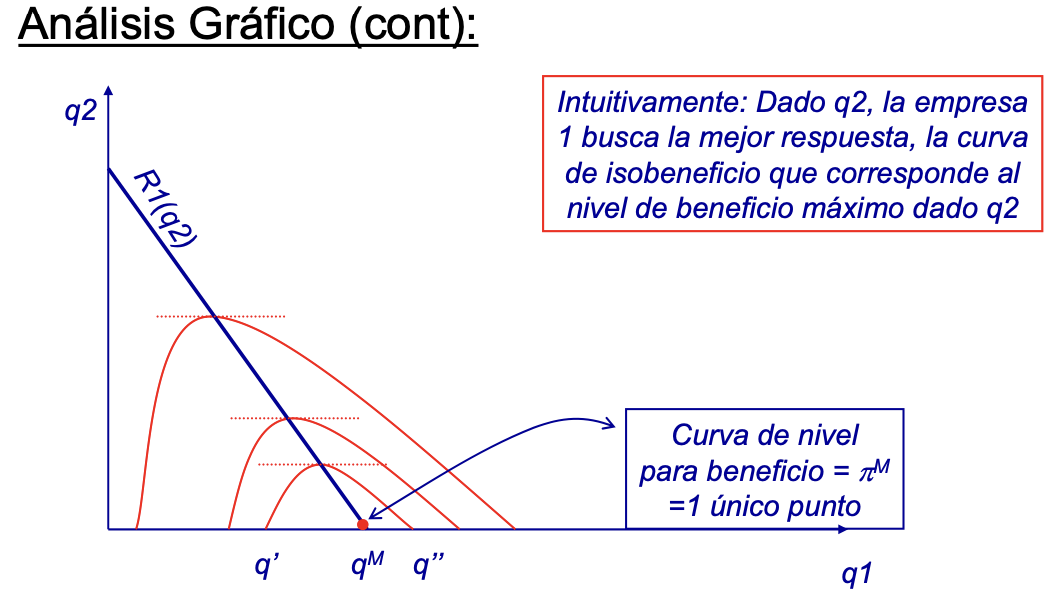
\includegraphics[width=10cm]{Captura de pantalla 2024-08-19 a la(s) 3.06.49 p. m..png}
        \end{center}
    \end{solution}

    \item[d)] Defina equilibrios de Nash y equilibrios perfecto en subjuegos. Cómo se relacionan.
    \begin{solution}
        Un equilibrio de Nash (EN) es un resultado de un juego (conjunto de estrategias) tal que ningún individuo tiene incentivo a cambiarla. 

        Un equilibrio perfecto en subjuegos (EPS) es un equilibrio de Nash creíble en un juego secuencial. 

        Todo EPS es un EN, pero no todo EN es un EPS. 
    \end{solution} 
    
    \item[e)] En un duopolio con competencia a la Cournot con un período finito, las empresas producen una cantidad equitativa para repartirse así las utilidades de monopolio. Dado que las utilidades de monopolio son las máximas posibles, las empresas decidirán mantener el acuerdo incluso si no se fuerza legalmente o de alguna otra manera. 
    \begin{solution}
        Sujeto a que la otra firma produce la mitad de lo que haría un monopolio, la estrategia óptima desde el punto de vista individual de la otra será producir más que la mitad de un monopolio. De esta manera el acuerdo no se mantiene sin un mecanismo de coacción. 

        Esto es valido para cualquier horizonte finito.
    \end{solution}
    \item[f)] ¿Hay alguna manera de que estas empresas decidan cooperar? Explique en que consiste el teorema de Folk.
    \begin{solution}
        El teorema de Folk nos indica que existe algun nivel de impaciencia (descuento) tal que un equilibrio cooperativo es factible en un juego repetido de horizonte infinito.

        Existe $0<\delta < 1$ tal que la utilidad de la cooperación es mayor a la utilidad de no cooperar.
        \begin{equation*}
            U_i = \sum_{t\geq 0} \delta^t u_i(x_t)
        \end{equation*}
    \end{solution}
\end{itemize}

\section{Juegos en forma extensiva}

Considere el siguiente juego secuencial en la figura 1.
\begin{figure}[h]
    \centering
    \caption{Juego en forma extensiva}
    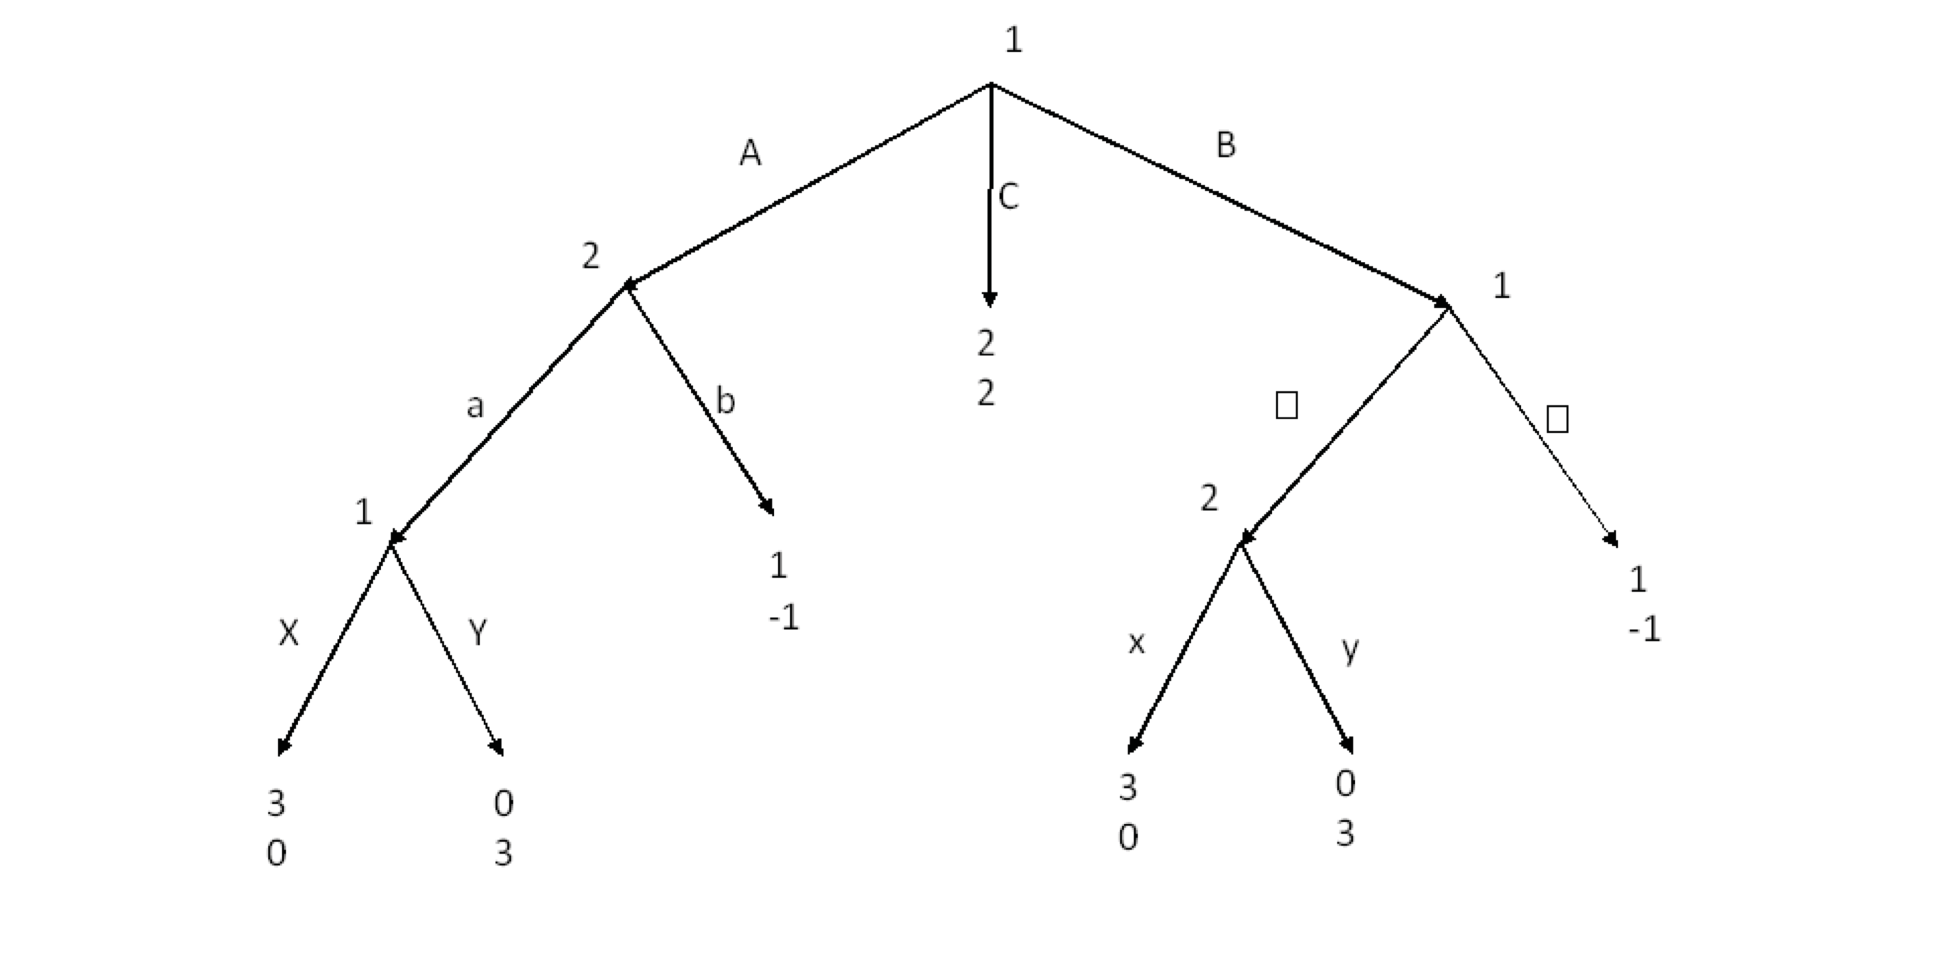
\includegraphics[width=10cm]{Captura de pantalla 2024-08-19 a la(s) 1.12.33 p. m..png}
\end{figure}
\begin{itemize}
    \item[a)] Encuentre el equilibrio de Nash.
    \begin{solution}
        Empezamos desde abajo. Para la parte inferior izquierda el jugador 1 escoge \( X \) para la parte inferior derecha el jugador 2 escoge \( y \). En la parte de al medio izquierda el jugador 2 escoge $a$, luego en la derech  el jugador 1 escoge $\beta$. Finalmente el jugador 1 escogerá $A$. 

        El equilibrio de Nash es \( (AX\beta, ay) \).
    \end{solution} 
    \item[b)] Escriba el juego en forma normal. 
    \begin{solution}
        \begin{center}
            \centering
            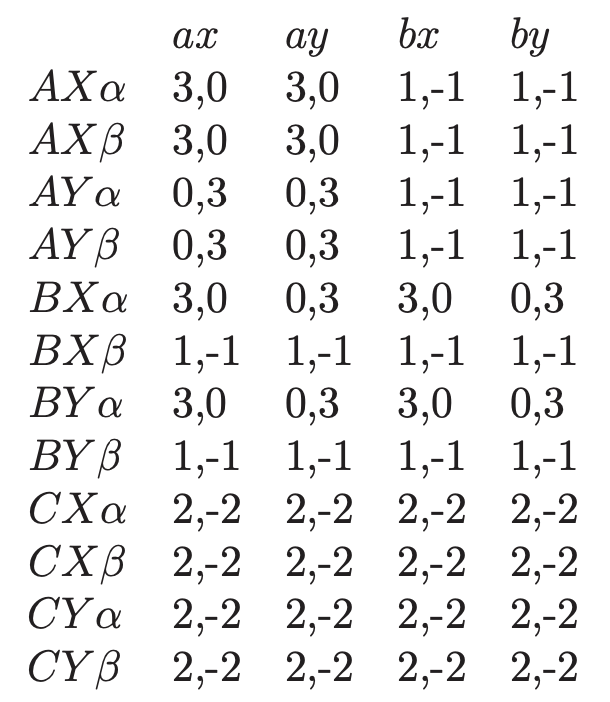
\includegraphics[width=5cm]{Captura de pantalla 2024-08-19 a la(s) 1.22.53 p. m..png}
        \end{center}
    \end{solution}
    \item[c)] Encuentre un equilibrio de Nash en forma normal que lleva a un resultado diferente al de la solución en a).
    \begin{solution}
        \( (CX\alpha, by) \) es otro equilibrio de Nash, esto ya que el jugador 2 no tiene incentivos de desviarse en caso de que el jugador 1 juegue \( C \) (literal acaba el juego). Mientras que el jugador 1 tampoco tiene incentivo para desviarse si juega $A$ el otro le resopnde con $b$ y gana 1. Si escoge $B$ entonces gana 0 o 1.
        
        Básicamente en forma normal el jugador 1 escoge $C$ y gana 2, pero en forma secuencial escoge $A$ puesto que sabe dada las estrategias creíbles acabará ganando 3.
    \end{solution}
\end{itemize}

\section{Stackelberg}

La curva de demanda inversa de un bien está dada por la función \( p(Q) = 240 - 2Q \). 
Existen dos firmas con las siguientes funciones de costos \( C_1(q_1) = 40q_1 \) 
y \( C_2(q_2) = 80q_2 \).

\begin{itemize}
    \item[a)] Si ambas firmas compiten a la Cournot. Determine las funciones de reacción de ambas. 
    ¿Cuál es el nivel de producción y el precio de equilibrio en este caso? 
    ¿Cuáles son los beneficios de ambas empresas?
\begin{solution}
    Firma 1 maximiza sus utilidades
    \begin{align*}
        \max_{q_1} \quad \Pi_1 = (240 - 2Q - 40)q_1 \\
        \frac{\partial \Pi_1}{\partial q_1} = (240 - 2q_2 - 4q_1 - 40) = 0 \\
        q_1^*(q_2) = \frac{200 - 2q_2}{4}
    \end{align*}
    Hacemos lo mismo para la firma 2.
    \begin{equation*}
        q_2^*(q_1) = \frac{160-2q_1}{4}
    \end{equation*}

    Reemplazamos uno en otro y tenemos que la firma 1 produce:
    \begin{align*}
        q_1 = \frac{200 - 2\left(\frac{160 - 2q_1}{4}\right)}{4}
    \end{align*}
    Los resultados son:
    \begin{align*}
        q_1^* = 40, \quad q_2^* = 20, \quad  p = 120 \\
        \Pi_1 = 3200, \quad \Pi_2 = 800
    \end{align*}

    
\end{solution}
\item[b)] Encuentré la expresión de la curva de isobeneficio de la firma 1, ¿que representa? Grafique.
\begin{solution}
    De manera genérica, 
    \begin{align*}
        \Pi_1 & (A-\eta (q_1 + q_2) - c_1)q_1 \\
        \bar{\pi}_1 =& Aq_1 - \eta q_1^2 - \eta q_1q_2 - c_1q_1 \\
        \eta q_1 q-2 =& (A-c)q_1 - \eta q_1^2 - \bar{\pi} \\
        q_2 =& \frac{A-c_1}{\eta} - q_1 - \frac{\bar{\pi}}{\eta q_1}
    \end{align*}
    Gráficos, \underline{\textbf{\href{https://www.geogebra.org/calculator/yzfrawqb}{Cournot con asimetría de costos}}}
\end{solution}

\item[c)] Suponga ahira que las dos empresas de la industria se comportan a la Stackelberg (en cantidad) de modo que la empresa 1 actúa como líder y la 2 como seguidora. ¿Cuál sería la producción y el precio de equilibrio de mercado? ¿Cuánto produciría la empresa 1? ¿Cuánto produciría la empresa 2? ¿Cuáles serán los beneficios de ambas empresas?
\begin{solution}
    Este es un juego secuencial en dos etapas, el cual se resuelve por inducción hacia atrás: En \( T = 2 \)
    \begin{align*}
        \max_{q_2} \quad \Pi_2 &= (240 - 2(q_1 + q_2))q_2 - 80q_2 \\
        \frac{\partial \Pi_2}{\partial q_2} &= (240 - 2q_1 - 4q_2 - 80) = 0 \\
        q^*_2(q_1) &= \frac{160 - 2q_1}{4}
    \end{align*}
    La firma 1 conoce la estrategia utilizada por la firma 2, por lo que escoge la cantidad óptima usando esta información.
    \begin{align*}
        \max_{q_1} \quad &\Pi_1 = (240 - 2(q_1 + q_2))q_1 - 40q_1 \\
        &s.a \quad q_2 = q_2(q_1) = \frac{160 - 2q_1}{4}
    \end{align*}
    Reemplazamos la restricción en la función objetivo.
    \begin{align*}
        \max_{q_1} \quad  \Pi_1=& (240 - 2(q_1 + \frac{160 - 2q_1}{4}))q_1 - 40q_1 \\
        \frac{\partial \Pi_1}{\partial q_1} =& 160 - 2q_1 - 40 = 0 \\
        q_1 =&60
    \end{align*}
    Por lo tanto, la mejor respuesta de la firma 2 será producir \( q_2 = 10 \). La producción total será \( Q^* = 70 \) y el precio será \( P^* = 100 \), luego, las utilidades serán:
    \[
    \Pi_1 = 3600, \quad \Pi_2 = 200
    \]

\end{solution}
\end{itemize}


\section{Propuesto: Colusión en Bertrand y Cournot}
Suponga que en China debido al coronavirus solo han quedado dos empresas que comercian animales exóticos para consumo. Ambas empresas tienen los mismos costos marginales, iguales a $c$, y venden un producto homogéneo. La demanda inversa de mercado que enfrentan está dada por $P=A-Q$. Las firmas están estudiando la posibilidad de coludirse en diferentes escenarios, para ello consideremos que las firmas descuentan los beneficios futuros a un factor $\delta$ y ante un desvío aplican la estrategia gatillo. Con esto se le pide que responda lo siguiente:

\begin{enumerate}
  \item Derive la condición que debe cumplir $\delta$ para que la colusión sea sostenible y encuentre el valor del factor $\delta^{C}$ que hace posible la colusión si estas firmas compiten en cantidades, y el factor $\delta^{B}$ que hace posible la colusión si estas firmas compiten en precios. Considere que al coludirse se reparten los beneficios equitativamente.
  \begin{solution}
    Considere la notación,
    \begin{itemize}
        \item $\pi^M$: Beneficios de monopolio.
        \item $\pi^C$: Beneficios de coludirse, también expresable en mayoría de los casos como $\pi^M/n$ siendo $n$ las empresas del mercado. 
        \item $\pi^N$: Beneficios de competir.
        \item $\pi^D$: Beneficios de desviarse.
    \end{itemize}
    Para que una estrategia colusiva sea sostenible, se debe cumplir que los beneficios de la colusión sea mayores o iguales a los de desvío y competencia.
    \begin{align*}
        VP(\text { colusión }) \geq VP(\text { desvío }) \\
        \sum_{i=0}^{\infty} \delta^{i} \pi^{C} \geq \pi^{D}+\sum_{i=1}^{\infty} \delta^{i} \pi^{N}
    \end{align*}
    Aplicamos la suma geométrica para llegar a un delta que cumpla la condición de colusión.
    \begin{align*}
        \frac{\pi^{C}}{1-\delta} &\geq \pi^{D}+\delta \frac{\pi^{N}}{1-\delta} \\
        \pi^{C} &\geq \pi^{D}(1-\delta)+\delta \pi^{N} \\
        \delta\left(\pi^{D}-\pi^{N}\right) &\geq \pi^{D}-\pi^{C} \\
        \delta &\geq \frac{\pi^{D}-\pi^{C}}{\pi^{D}-\pi^{N}}
    \end{align*}
    Solo hace falta calcular los pagos para cada caso y así encontrar el $\delta$ mínimo que cumpla la condición. Los pagos dependerán de la competencia así que vamos caso por caso.

    \rule{\linewidth}{0.4pt} 
    \textbf{Bertrand} 
    
    Los beneficios de coludirse bajo competencia en precios son los beneficios monopólicos repartidos en ambas firmas.
    \begin{align*}
        \pi^{C}= \frac{\pi^{M}}{2}= \frac{(A-c)^{2}}{8}
    \end{align*}
    Los beneficios de desvío son iguales a los beneficios monopólicos. 
    \begin{align*}
        \pi^{D}=\pi^{M}=\frac{(A-c)^{2}}{4}
    \end{align*}
    Y los beneficios de no cooperar son $\pi^{N}=0$. Luego, reemplazando en la condición de colusión.
    \begin{align*}
        \delta^{B}=\frac{\pi^{D}-\pi^{C}}{\pi^{D}-\pi^{N}}=\frac{\frac{(A-c)^{2}}{4}-\frac{(A-c)^{2}}{8}}{\frac{(A-c)^{2}}{4}-0}=\frac{\frac{(A-c)^{2}}{8}}{\frac{(A-c)^{2}}{4}}=\frac{1}{2} \\
        \delta^{B}=\frac{1}{2}
    \end{align*}

    \rule{\linewidth}{0.4pt} 
    \textbf{Cournot}
    
    Los beneficios colusivos son iguales al caso de competencia en precios.
    \begin{align*}
        \pi^{C}=\frac{\pi^{M}}{2}=\frac{(A-c)^{2}}{8}
    \end{align*}
    Luego, los beneficios de competir los obtenemos de la siguiente forma. Primero, de la maximización de la firma $i$, obtenemos la función de reacción de la firma $i$.
    \begin{equation*}
        q_{i}=\frac{A-q_{j}-c}{2}
    \end{equation*} 
    Luego, la cantidad que produce cada firma es $q_{i}=\frac{A-c}{3}$, la cantidad total $Q=\frac{2(A-c)}{3}$ y el precio $P=\frac{A+2 c}{3}$. Entonces los beneficios no colusivos son
    \begin{equation*}
        \pi^{N}=\frac{(A-c)^{2}}{9}
    \end{equation*} Para calcular los beneficios de desvío reemplazamos la cantidad colusiva de la firma $i$ en la función de reacción de la firma $j$.
    \begin{align*}
        q_{j}^{D}=\frac{A-q_{i}^{C}-c}{2}=\frac{A-\frac{A-c}{4}-c}{2}=\frac{3(A-c)}{8}
    \end{align*}
    Los beneficios de desviarse son
    \begin{align*}
        \pi^{D}=\frac{9(A-c)^{2}}{64}
    \end{align*}
    Finalmente reemplazamos en la condición de colusión.
    \begin{align*}
        \delta^{C}=\frac{\pi^{D}-\pi^{C}}{\pi^{C}-\pi^{N}}=\frac{\frac{9(A-c)^{2}}{64}-\frac{(A-c)^{2}}{8}}{\frac{9(A-c)^{2}}{64}-\frac{(A-c)^{2}}{9}} \\
        \delta^{C} \geq \frac{9}{17} \approx 0,53
    \end{align*}
  \end{solution}
    \item ¿Bajo que tipo de competencia es más factible la colusión?

    \begin{solution}
    De la parte anterior se tiene que $\delta^{C}>\delta^{B}$ por lo tanto es más fácil coludirse en Bertrand debido a que el castigo es más severo que en Cournot.
    \end{solution}
\end{enumerate}

\section{Propuesto: Stackelberg con inversión}

Considere una industria con dos empresas, L y S, que producen un producto homogéneo. 
La empresa L es la líder y la S la seguidora. La función inversa de demanda, \( p(Q) \), 
es igual \( p(q_L, q_S) = 1 - q_L - q_S \), donde \( q_L \) y \( q_S \) son las cantidades 
producidas por la líder y la seguidora, respectivamente, y \( p \) es el precio de mercado. 
Suponga, además, que la función de costes es \( C_i(q_i) = \frac{1}{2} q_i \), para \( i = L, S \).

\begin{enumerate}
    \item[(a)] Calcule las producciones en equilibrio, el precio de mercado, las cuotas de mercado, y el beneficio de cada empresa.
    \item[(b)] Suponga que las empresas compiten en cantidades simultáneamente (Cournot). 
    Calcule las cantidades de equilibrio, el precio, las cuotas y los beneficios, y compare su respuesta con la anterior.
    \item[(c)] Suponga que las empresas compiten en cantidades secuencialmente, 
    pero ahora la empresa \( S \) puede invertir \( \bar{S} \) y convertirse en líder. 
    ¿Debería la seguidora invertir? ¿Cómo depende su decisión del valor de S?
\end{enumerate}

\end{document}